\documentclass[aspectratio=169,10pt]{beamer}

\usetheme[progressbar=frametitle, block=fill]{metropolis}

\usepackage{amsmath,amssymb}
\usepackage{graphicx}
\usepackage{booktabs}
\usepackage{multirow}
\usepackage{xcolor}
\usepackage{colortbl}

% ── colours ──────────────────────────────────────────────────────────────────
\definecolor{accent}{RGB}{30,80,160}
\definecolor{lightgray}{RGB}{245,245,245}
\setbeamercolor{frametitle}{bg=accent}
\setbeamercolor{progress bar}{fg=accent}
\setbeamercolor{alerted text}{fg=accent}

% ── macros ───────────────────────────────────────────────────────────────────
\def\fm#1{\mathcal{#1}}
\newcommand{\bcirc}{\mathrm{bcirc}}
\newcommand{\highlight}[1]{\textcolor{accent}{\textbf{#1}}}

% ── title ────────────────────────────────────────────────────────────────────
\title{TGDBEK}
\subtitle{Tensor Greedy Double Block Extended Kaczmarz\\
          for Inconsistent Tensor Linear Systems}
\author{Jeremie Mabiala}
\institute{AIMS / AMMI, Senegal}
\date{\today}

% =============================================================================
\begin{document}
% =============================================================================

\maketitle

% ── 1. What problem are we solving? ──────────────────────────────────────────
\begin{frame}{What problem are we solving?}

  \begin{columns}[T]
    \column{0.55\textwidth}
      We want to solve a \textbf{large, noisy tensor system}:
      \[
        \fm{A} \;*\; \fm{X} \;=\; \fm{B} + \varepsilon
      \]
      \vspace{4pt}
      \begin{itemize}
        \item $\fm{A}, \fm{B}, \fm{X}$ are \textbf{third-order tensors}
        \item $*$ is the \textbf{t-product} (Kilmer et al., 2011)
        \item The system is \textbf{inconsistent} because of noise $\varepsilon$
        \item Target: the \textbf{minimum-norm least-squares} solution
              $\fm{X}_* = \fm{A}^\dagger * \fm{B}$
      \end{itemize}

    \column{0.42\textwidth}
      \begin{center}
        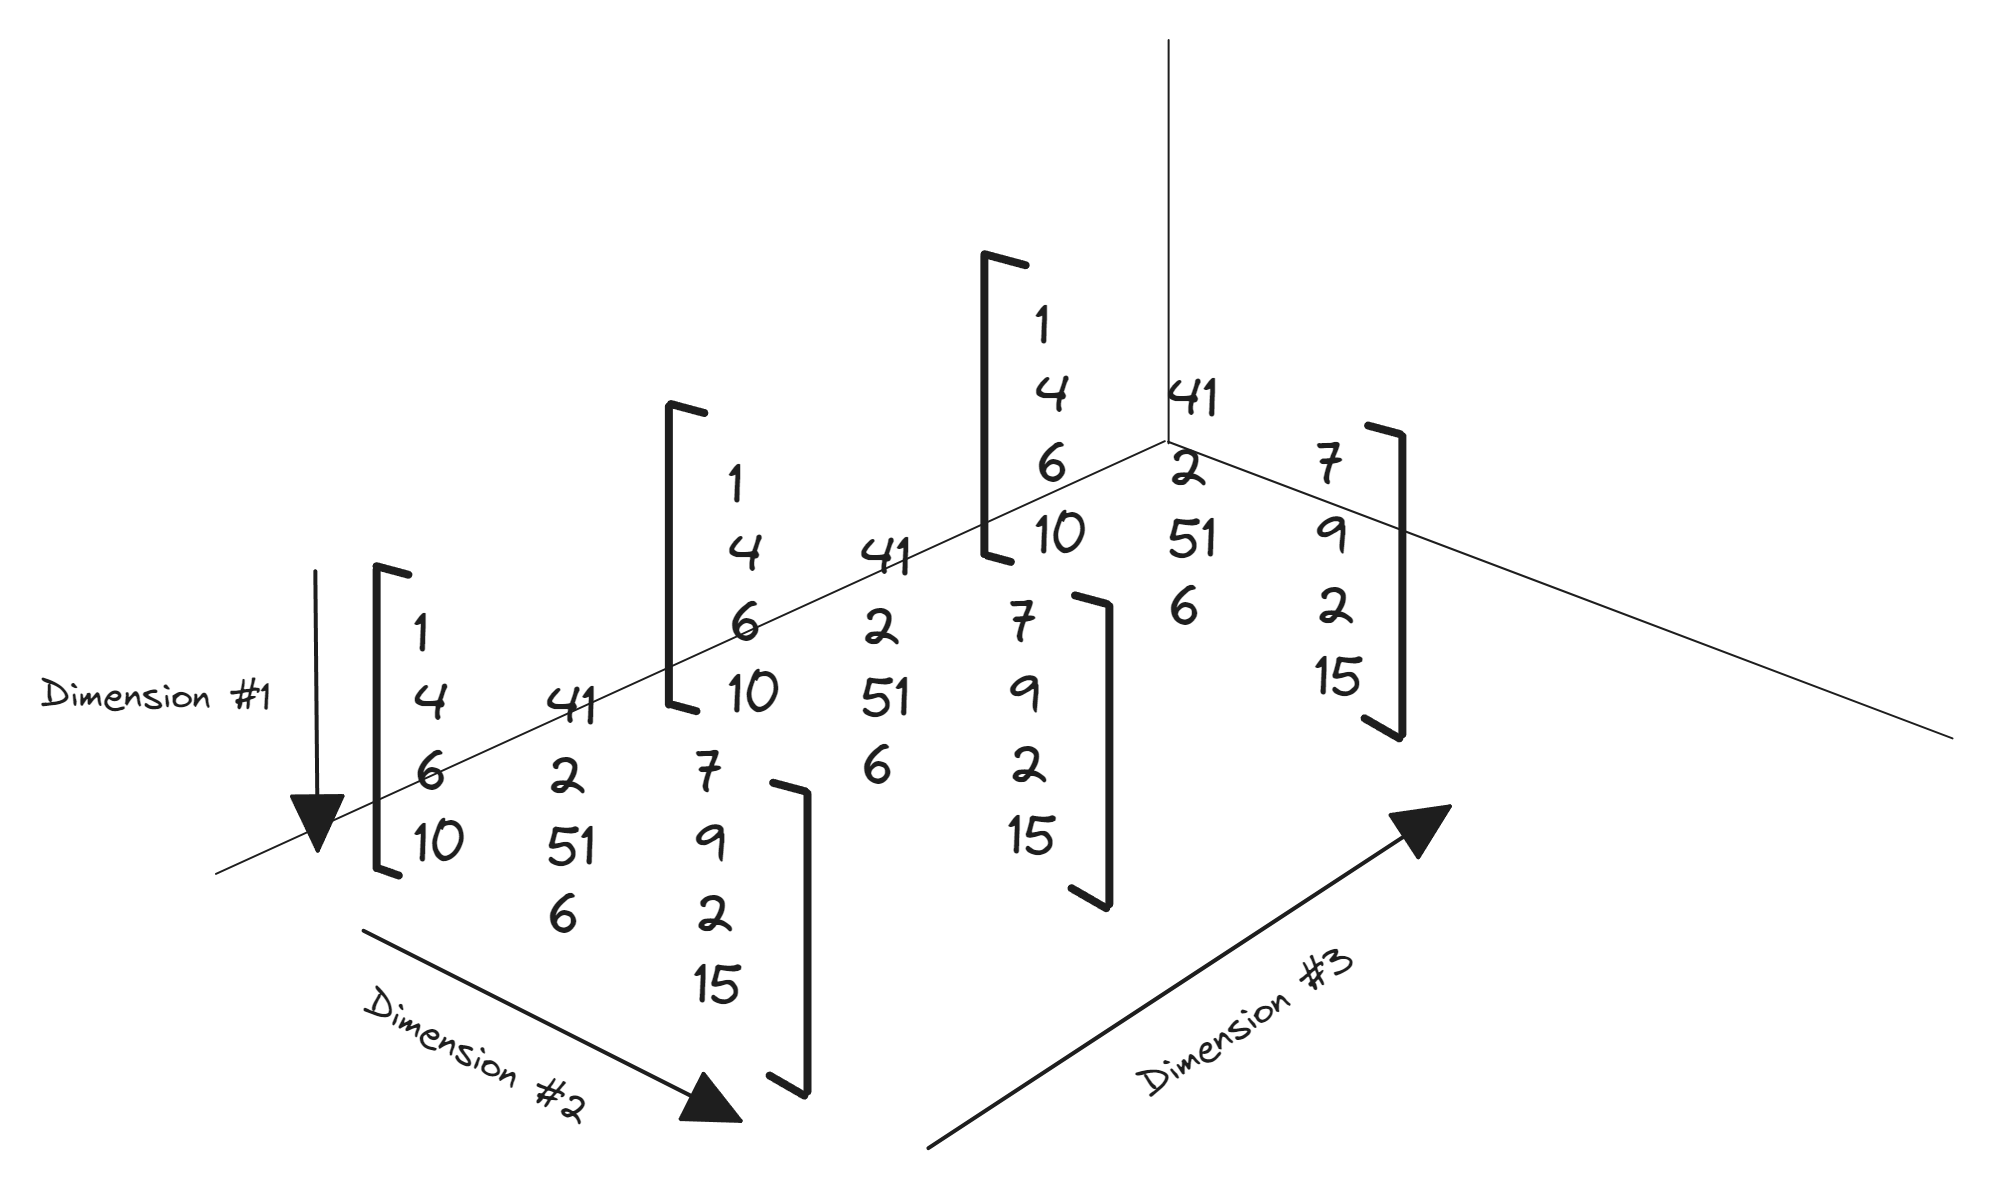
\includegraphics[width=0.85\linewidth]{slides-images/3d-tensor-2.png}
      \end{center}
      \vspace{4pt}
      \small\centering
      \textbf{Applications:} color image deblurring,\\
      MRI reconstruction, multi-channel data
  \end{columns}

\end{frame}

% ── 2. The t-product in one slide ─────────────────────────────────────────────
\begin{frame}{The t-product: matrix algebra lifted to tensors}

  \begin{columns}[T]
    \column{0.50\textwidth}
      A third-order tensor $\fm{A} \in \mathbb{R}^{N_1 \times N_2 \times N_3}$
      has frontal slices $A_1, \ldots, A_{N_3}$.

      \medskip
      The \textbf{t-product} $\fm{A} * \fm{B}$ is defined via the
      \emph{block-circulant matrix}:
      \[
        \bcirc(\fm{A}) =
        \begin{pmatrix}
          A_1 & A_{N_3} & \cdots & A_2 \\
          A_2 & A_1     & \cdots & A_3 \\
          \vdots & & \ddots & \vdots \\
          A_{N_3} & \cdots & \cdots & A_1
        \end{pmatrix}
      \]

    \column{0.46\textwidth}
      \begin{alertblock}{Why this matters}
        The t-product gives tensors the \emph{same algebra as matrices}:
        \begin{itemize}
          \item Transpose, inverse, pseudoinverse $\fm{A}^\dagger$
          \item Frobenius \& spectral norms
          \item Orthogonal projectors
        \end{itemize}
        $\Rightarrow$ We can run \textbf{Kaczmarz-type iterations} directly
        on the tensor system.
      \end{alertblock}
  \end{columns}

\end{frame}

% ── 3. Existing methods and their limitation ──────────────────────────────────
\begin{frame}{Existing methods — and the gap}

  \begin{center}
  \small
  \begin{tabular}{lcc}
    \toprule
    Method & Handles inconsistency? & Needs fixed partitions? \\
    \midrule
    TREK  (Huang et al., 2023)   & \textcolor{green!60!black}{\textbf{Yes}} & \textcolor{green!60!black}{\textbf{No}} \\
    TREBK (Huang et al., 2023)   & \textcolor{green!60!black}{\textbf{Yes}} & \textcolor{red}{\textbf{Yes}} \\
    TREGBK (Huang et al., 2023)  & \textcolor{green!60!black}{\textbf{Yes}} & \textcolor{red}{\textbf{Yes}} \\
    TREABK (An et al., 2024)     & \textcolor{green!60!black}{\textbf{Yes}} & \textcolor{red}{\textbf{Yes}} \\
    \midrule
    \highlight{TGDBEK (ours)}    & \textcolor{green!60!black}{\textbf{Yes}} & \textcolor{green!60!black}{\textbf{No}} \\
    \bottomrule
  \end{tabular}
  \end{center}

  \bigskip
  \begin{alertblock}{The problem with fixed partitions}
    TREBK, TREGBK, TREABK all require the user to \emph{pre-split} rows and
    columns of the system into blocks before running.  This is
    \textbf{problem-dependent}, and performs poorly on \textbf{heterogeneous or
    sparse tensors} where the natural block structure is unknown.
  \end{alertblock}

\end{frame}

% ── 4. Our idea ───────────────────────────────────────────────────────────────
\begin{frame}{Our idea: let the residual choose the blocks}

  \textbf{Key insight.} At each iteration, instead of using fixed partitions,
  we \emph{greedily} pick the rows and columns with the \textbf{largest residual}.

  \bigskip
  \begin{columns}[T]
    \column{0.48\textwidth}
      \begin{block}{Z-step — push $\fm{Z}$ to null$(\fm{A}^\top)$}
        Select column blocks $U_k$ where
        \[
          \frac{\|\fm{A}_{:,j,:}^\top * \fm{Z}^{(k)}\|_F^2}
               {\|\fm{A}_{:,j,:}\|_F^2}
          \;\geq\; \eta \cdot \max_j(\cdots)
        \]
        Update: $\fm{Z}^{(k+1)} = \fm{Z}^{(k)} - \fm{A}_{:,U_k,:} *
        (\fm{A}_{:,U_k,:})^\dagger * \fm{Z}^{(k)}$
      \end{block}

    \column{0.48\textwidth}
      \begin{block}{X-step — push $\fm{X}$ to least-squares solution}
        Select row blocks $J_k$ where residual is largest, then update:
        \[
          \fm{X}^{(k+1)} = \fm{X}^{(k)} + (\fm{A}_{J_k,:,:})^\dagger *
          \bigl(\fm{B}_{J_k} - \fm{Z}^{(k+1)}_{J_k} - \fm{A}_{J_k}*\fm{X}^{(k)}\bigr)
        \]
      \end{block}
  \end{columns}

  \bigskip
  \begin{itemize}
    \item $\eta \in (0,1]$ — threshold controlling how many blocks are selected
    \item \textbf{No partition needed}: the active sets $U_k$, $J_k$ are built fresh each step
  \end{itemize}

\end{frame}

% ── 5. What we prove ──────────────────────────────────────────────────────────
\begin{frame}{What we prove}

  \begin{block}{Theorem (linear convergence)}
    The iterates $\{\fm{X}^{(k)}\}$ of TGDBEK satisfy
    \[
      \|\fm{X}^{(k)} - \fm{X}_*\|_F^2
      \;\leq\;
      \alpha^k \|\fm{X}^{(0)} - \fm{X}_*\|_F^2 \;+\; C \cdot \beta^k
    \]
    for constants $\alpha, \beta \in (0,1)$ depending on $\eta$ and the
    singular values of $\fm{A}$.
    The iterates converge \textbf{linearly} to the minimum-norm
    least-squares solution $\fm{X}_* = \fm{A}^\dagger * \fm{B}$.
  \end{block}

  \bigskip
  \textbf{How the proof works:}
  \begin{enumerate}
    \item The Z-step is an orthogonal projection $\Rightarrow$ contracts
          $\|\fm{Z}^{(k)} - \fm{B}^\perp\|_F$ by factor $\beta < 1$ per step.
    \item The greedy row selection ensures the X-step always makes progress
          $\Rightarrow$ contracts $\|\fm{X}^{(k)} - \fm{X}_*\|_F$ by $\alpha < 1$.
    \item Combining the two gives the coupled linear recurrence above.
  \end{enumerate}

\end{frame}

% ── 6. Dense systems ──────────────────────────────────────────────────────────
\begin{frame}{Result 1 — Dense overdetermined systems}

  $\fm{A}\in\mathbb{R}^{500 \times n \times 10}$, varying $n$, noise $a=10^{-3}$

  \begin{columns}[T]
    \column{0.50\textwidth}
      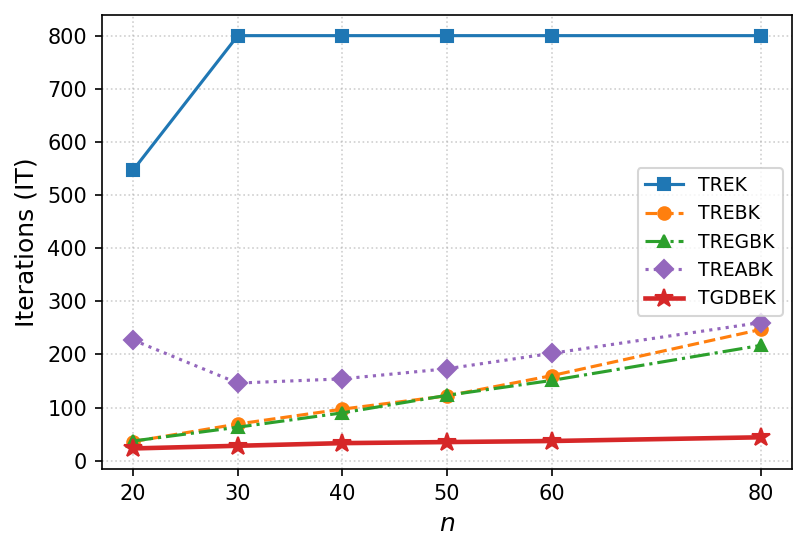
\includegraphics[width=\linewidth]{main-folder/tests/tests/ex1-IT.png}

    \column{0.47\textwidth}
      \small
      \begin{tabular}{lrr}
        \toprule
        Method & IT ($n{=}80$) & Converges? \\
        \midrule
        TREK            & 800 (budget) & \textcolor{red}{\textbf{No}} \\
        TREBK           & 247          & \textcolor{green!60!black}{\textbf{Yes}} \\
        TREGBK          & 217          & \textcolor{green!60!black}{\textbf{Yes}} \\
        \textbf{TGDBEK} & \textbf{44}  & \textcolor{green!60!black}{\textbf{Yes}} \\
        \bottomrule
      \end{tabular}

      \bigskip
      \begin{itemize}
        \item \highlight{Up to 16$\times$ fewer iterations} than TREK
        \item \highlight{3--5$\times$ fewer} than TREBK / TREGBK
        \item TREK \emph{never converges} for $n \geq 30$
      \end{itemize}
  \end{columns}

\end{frame}

% ── 7. Image deblurring ───────────────────────────────────────────────────────
\begin{frame}{Result 2 — Color image deblurring}

  $200\times200\times3$ image, Gaussian blur $\sigma=4$, noise $a=10^{-2}$, max 1000 iterations

  \begin{columns}[T]
    \column{0.55\textwidth}
      \begin{center}
      \small
      \begin{tabular}{ccc}
        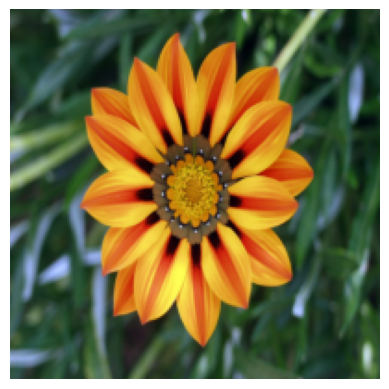
\includegraphics[width=0.28\linewidth]{main-folder/tests/tests/ex3-origin-after-resh.png} &
        
\includegraphics[width=0.28\linewidth]{main-folder/tests/tests/ex3-blur.png} &
        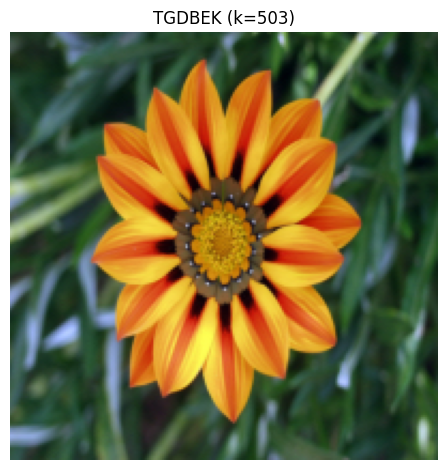
\includegraphics[width=0.28\linewidth]{main-folder/tests/tests/ex3-tgdbek.png} \\
        True & Blurred+noisy & \textbf{TGDBEK} \\
      \end{tabular}
      \end{center}

      \begin{center}
      \small
      \begin{tabular}{cc}
        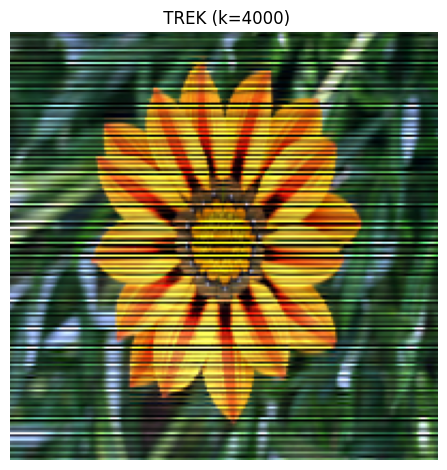
\includegraphics[width=0.28\linewidth]{main-folder/tests/tests/ex3-trek.png} &
        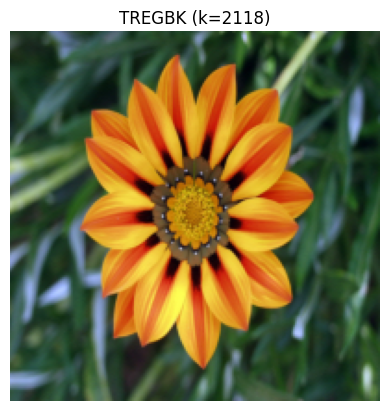
\includegraphics[width=0.28\linewidth]{main-folder/tests/tests/ex3-tregbk.png} \\
        TREK (stagnates) & TREGBK (stagnates) \\
      \end{tabular}
      \end{center}

    \column{0.42\textwidth}
      \small
      \begin{tabular}{lrr}
        \toprule
        Method & IT & RSE \\
        \midrule
        TREK   & 1000 & $7.9\times10^{-1}$ \\
        TREBK  & 1000 & $2.2\times10^{-2}$ \\
        TREGBK & 1000 & $1.3\times10^{-3}$ \\
        \textbf{TGDBEK} & \textbf{503} & $\mathbf{1.0\times10^{-5}}$ \\
        \bottomrule
      \end{tabular}

      \bigskip
      \highlight{Only TGDBEK converges}\\
      within the 1000-iteration budget.

      \bigskip
      PSNR $\approx 30.3\,$dB,\; SSIM $\approx 0.843$
  \end{columns}

\end{frame}

% ── 8. High-iteration / MRI ───────────────────────────────────────────────────
\begin{frame}{Result 3 — Harder regime \& MRI-like reconstruction}

  \begin{columns}[T]
    \column{0.48\textwidth}
      \textbf{High-iteration image deblurring}\\
      (noise $a=10^{-1}$, max 3000 iterations)

      \medskip
      \small
      \begin{tabular}{lrr}
        \toprule
        Method & IT & CPU (s) \\
        \midrule
        TREK            & 3000 & 10.7 \\
        TREBK           & 2363 & 21.7 \\
        TREGBK          & 1730 & 31.6 \\
        \textbf{TGDBEK} & \textbf{502} & \textbf{18.5} \\
        \bottomrule
      \end{tabular}

      \medskip
      \highlight{42\% faster wall time} than TREGBK\\
      at one-third the iterations

    \column{0.48\textwidth}
      \textbf{Shepp-Logan MRI phantom}\\
      ($128\times128\times27$, noise $a=10^{-3}$)

      \begin{center}
      \small
      \begin{tabular}{cc}
        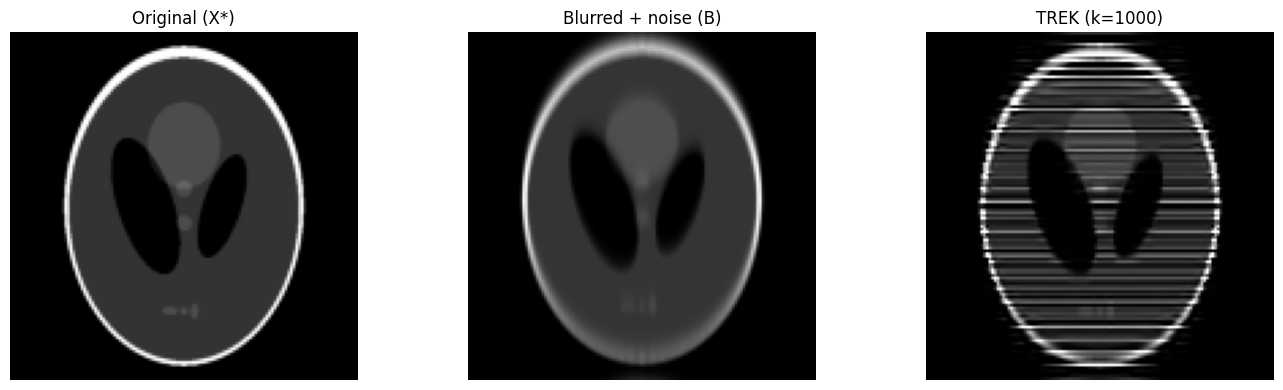
\includegraphics[width=0.38\linewidth]{main-folder/tests/tests/gray-trek.png} &
        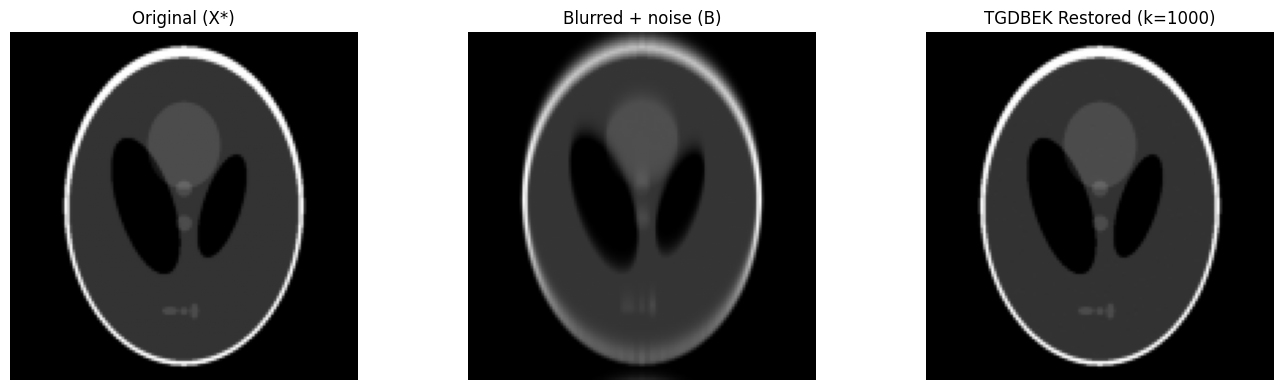
\includegraphics[width=0.38\linewidth]{main-folder/tests/tests/gray-tgdbek.png} \\
        TREK & \textbf{TGDBEK} \\
        18.1\,dB & \textbf{58.0\,dB} \\
      \end{tabular}
      \end{center}

      \medskip
      TREABK diverges (NaN). TGDBEK matches best\\
      quality (TREGBK) with lower CPU.
  \end{columns}

\end{frame}

% ── 9. Summary ────────────────────────────────────────────────────────────────
\begin{frame}{Summary}

  \begin{columns}[T]
    \column{0.50\textwidth}
      \textbf{What TGDBEK is:}
      \begin{itemize}
        \item An iterative solver for \emph{inconsistent} tensor linear systems
        \item Greedy block selection — \emph{no user-defined partitions}
        \item Provably convergent to $\fm{X}_* = \fm{A}^\dagger*\fm{B}$
      \end{itemize}

      \bigskip
      \textbf{Main improvements over prior methods:}
      \begin{itemize}
        \item Up to \highlight{16$\times$ fewer iterations} (vs.\ TREK)
        \item Up to \highlight{5$\times$ fewer iterations} (vs.\ TREBK/TREGBK)
        \item \highlight{Only method to converge} on color image deblurring (1000-iter budget)
        \item \highlight{42\% wall-time reduction} on hard imaging problem
        \item Numerically \highlight{stable where TREABK diverges}
      \end{itemize}

    \column{0.46\textwidth}
      \textbf{Future directions:}
      \begin{enumerate}
        \item Adaptive $\eta$ during iteration
        \item Randomized + greedy hybrid
        \item Higher-order tensors
        \item Tighter convergence rate bounds
      \end{enumerate}

      \bigskip
      \textbf{Code:}\\
      \small\url{https://github.com/jnlandu/tensor-greedy-double-extended-kaczmarz}
  \end{columns}

  \bigskip\bigskip
  \begin{center}
    \large\textbf{Thank you — Questions?}
  \end{center}

\end{frame}

\end{document}
